    \chapter*{Introduction to Hardware and Software components}
    This chapter serves as an introduction to the frameworks, software, and libraries we use. The work we present can be simplified explained as a knowledge base containing parameters that a robot can use to perform specific actions.

    Firstly, we would like to introduce the robotic component, which acts as the interface between the knowledge base we have created and the robot, followed by an introduction to Ontologies and Knowledgebases.
        \section*{Robotic section: ROS and PyCram}
    
    The main framework we use is PyCram, which serves as an interface for various software components such as knowledge, perception, or manipulation. This framework utilizes another framework, ROS, to communicate with the different robot components. These two frameworks are now introduced in the following.    
    \subsection*{ROS}
    \begin{wrapfigure}{r}{0.5\textwidth}
        \centering
        
\includegraphics[width=0.48\textwidth]{Graphics/ROS.jpg}
    \end{wrapfigure}
    ROS, which stands for Robot Operating System, is an open-source middleware framework designed to develop and control robots. Despite its name, ROS is not a traditional operating system but rather a set of software libraries and tools that help in building and managing robot software. It provides a standardized and modular approach to developing robotic systems, allowing for easier collaboration and code reuse in the robotics community.
    Key features and components of ROS include:
    \begin{itemize}
        \item Nodes: ROS systems are organized into nodes, which are individual processes that perform specific tasks. Nodes communicate with each other by passing messages over topics, creating a decentralized and modular architecture.
        \item Topics: Nodes exchange data through topics, which are named buses over which messages are passed. This publish/subscribe communication model allows for asynchronous and loosely coupled interactions between nodes.
        \item Launch files: ROS uses launch files to specify how to start multiple nodes and configure the system. This helps simplify the setup of complex robotic systems.
        \item Master: The ROS Master is responsible for managing the communication between nodes by keeping track of publishers, subscribers, and services. It facilitates the discovery and connection of nodes within a ROS network.
    \end{itemize}

    \subsection*{Pr2}
	Introduced in 2010 by Willow Garage (https://robotsguide.com/robots/pr2), the PR2 stands as an advanced research robot. Boasting multiple joints and 20 degrees of freedom, this robot excels in autonomous navigation and the manipulation of a diverse array of objects, making it an ideal choice for our specific needs. Additionally, it is equipped with a HeadStereoCamera that can be used to perceive the surroundings.
	
    \begin{figure}[H]
    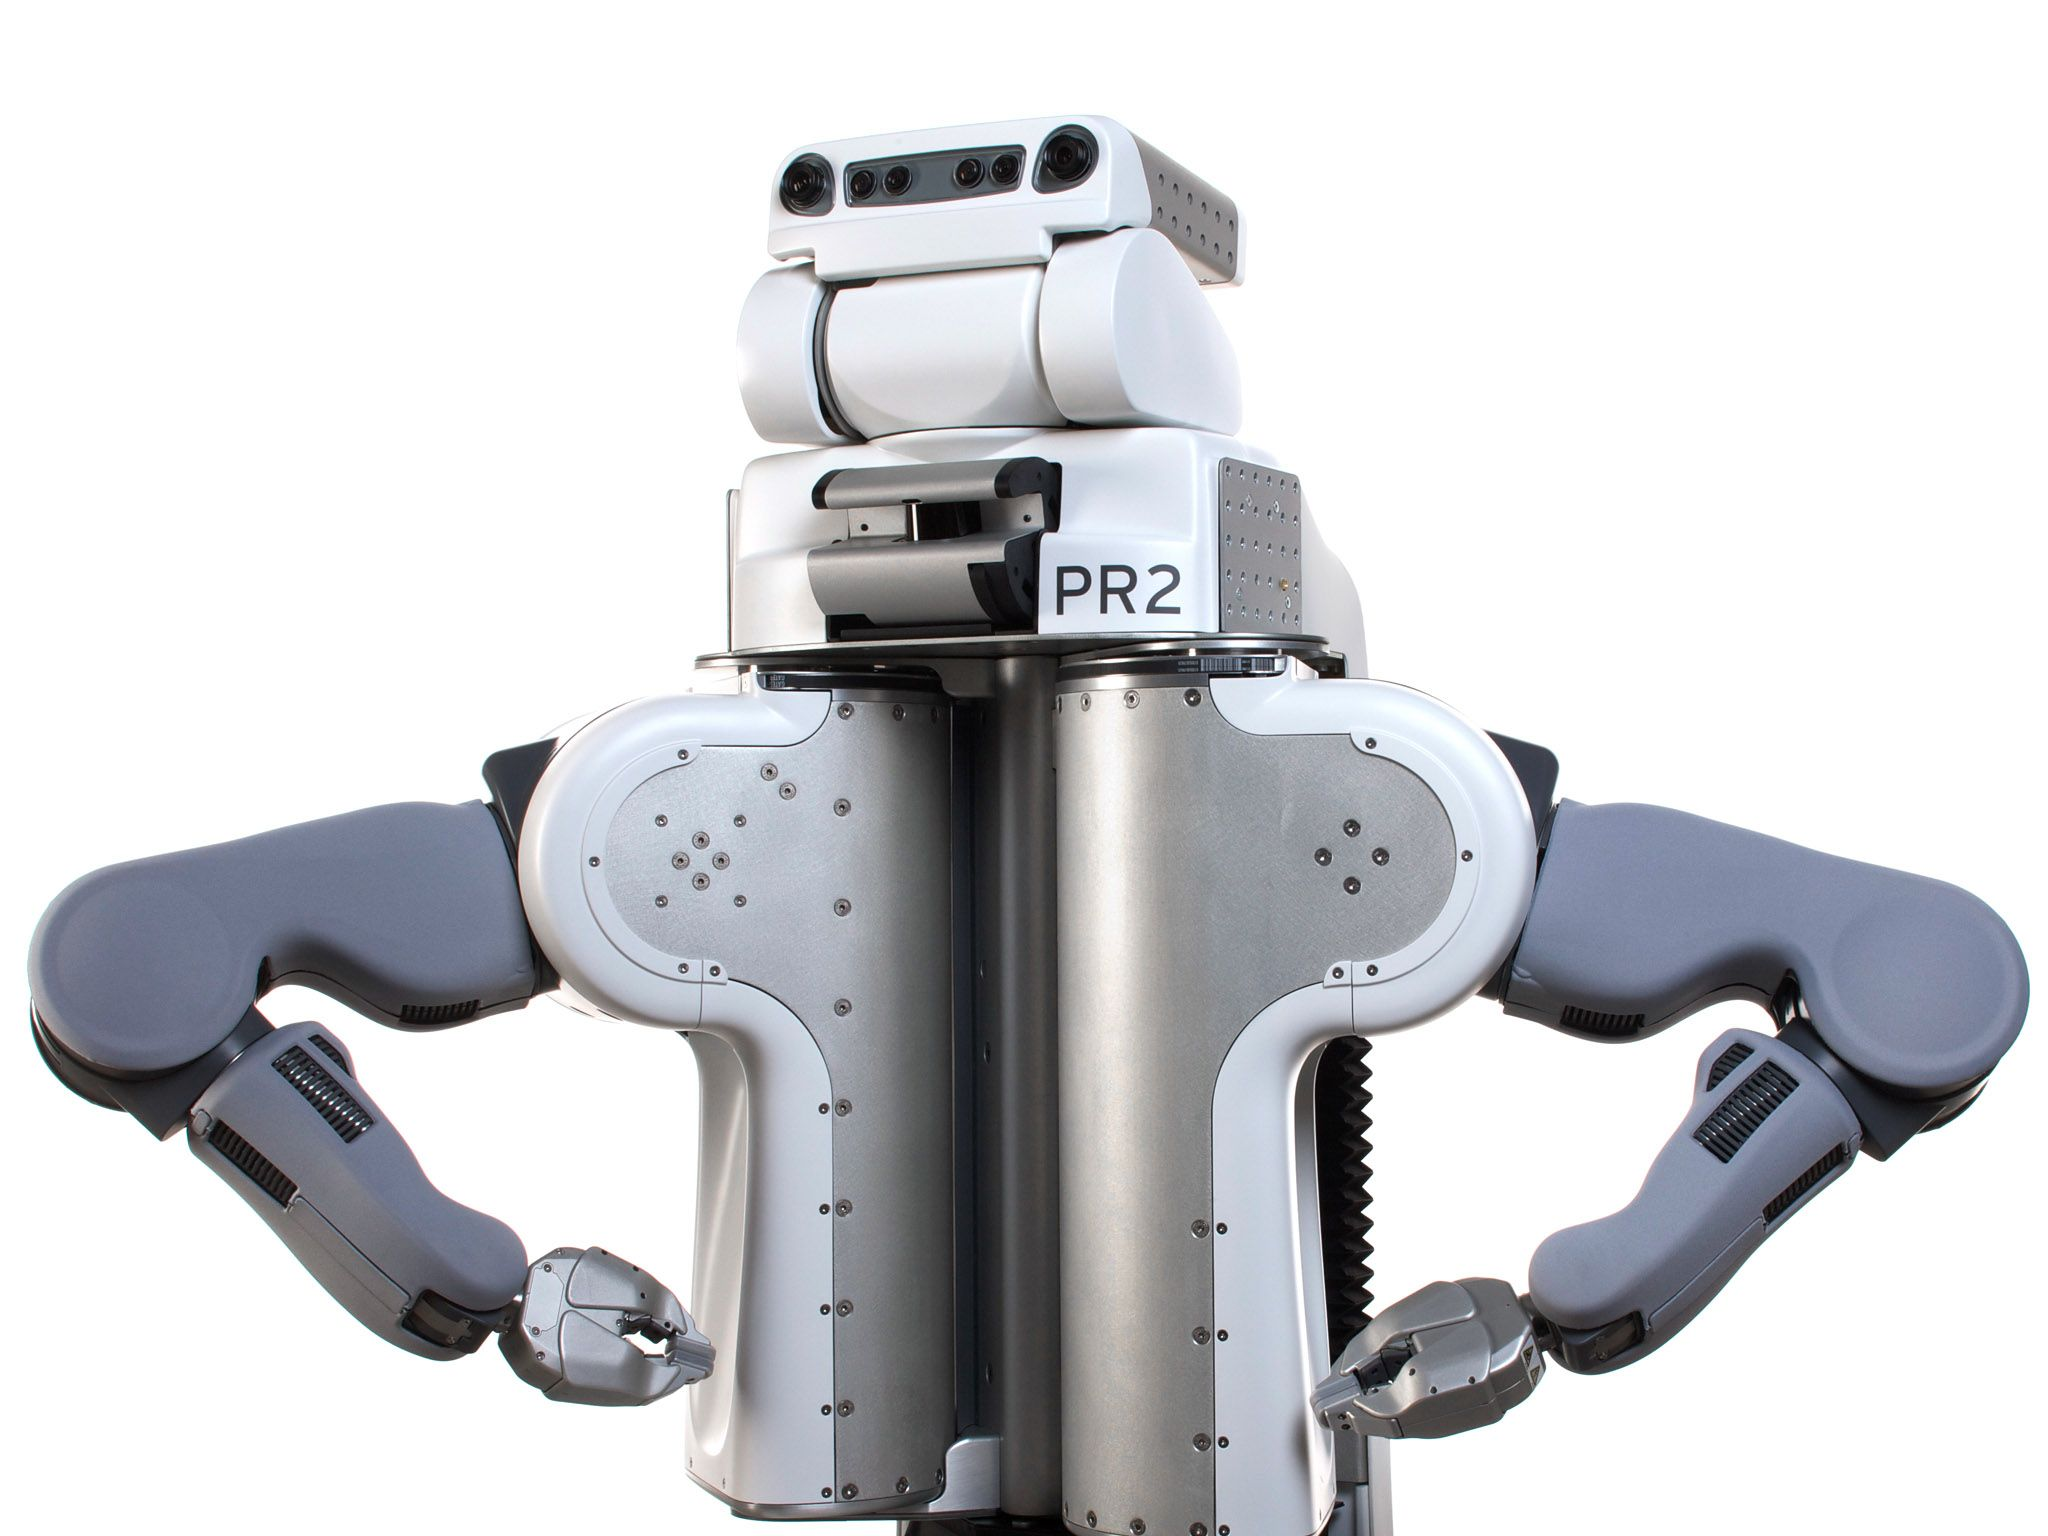
\includegraphics[scale=0.1]{Graphics/pr2.jpg}
    \end{figure}
    \subsection*{PyCram}
    VON PYCRAM:
	PyCRAM is a toolbox for designing, implementing and deploying software on autonomous robots. The framework provides various tools and libraries for aiding in robot software development as well as geometric reasoning and fast simulation mechanisms to develop cognition-enabled control programs that achieve high levels of robot autonomy.
    PyCRAM is developed in Python with support for the ROS middleware which is used for communication with different software components as well as the robot.
    
    VON CRAM: CRAM (Cognitive Robot Abstract Machine) is a software toolbox for the design, the implementation, and the deployment of cognition-enabled autonomous robots performing everyday manipulation activities. CRAM equips autonomous robots with lightweight reasoning mechanisms that can infer control decisions rather than requiring the decisions to be pre-programmed. This way CRAM-programmed autonomous robots are much more flexible, reliable, and general than control programs that lack such cognitive capabilities. CRAM does not require the whole domain to be stated explicitly in an abstract knowledge base. Rather, it grounds symbolic expressions in the knowledge representation into the perception and actuation routines and into the essential data structures of the control programs. 

    \begin{figure}[H]
    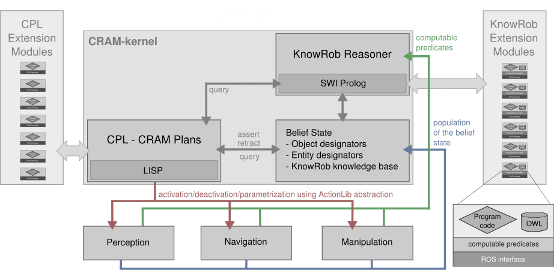
\includegraphics[scale=1.5]{Graphics/cram-language-architecture.png}
    \end{figure}
    \section*{Knowledge Section: Ontologies and Rules}
    The parameters inferred for various robot actions come from a knowledge base. In the following, the principle of an ontology, as well as the concept of rules, which play a crucial role in parameter inference, will be introduced.
    \subsection*{Ontology}
	Ontologies are structured frameworks that provide a formal representation of knowledge within a specific domain. They play a crucial role in knowledge representation, facilitating the organization and sharing of information in a way that is both machine-readable and understandable by humans. 

    \begin{figure}[H]
        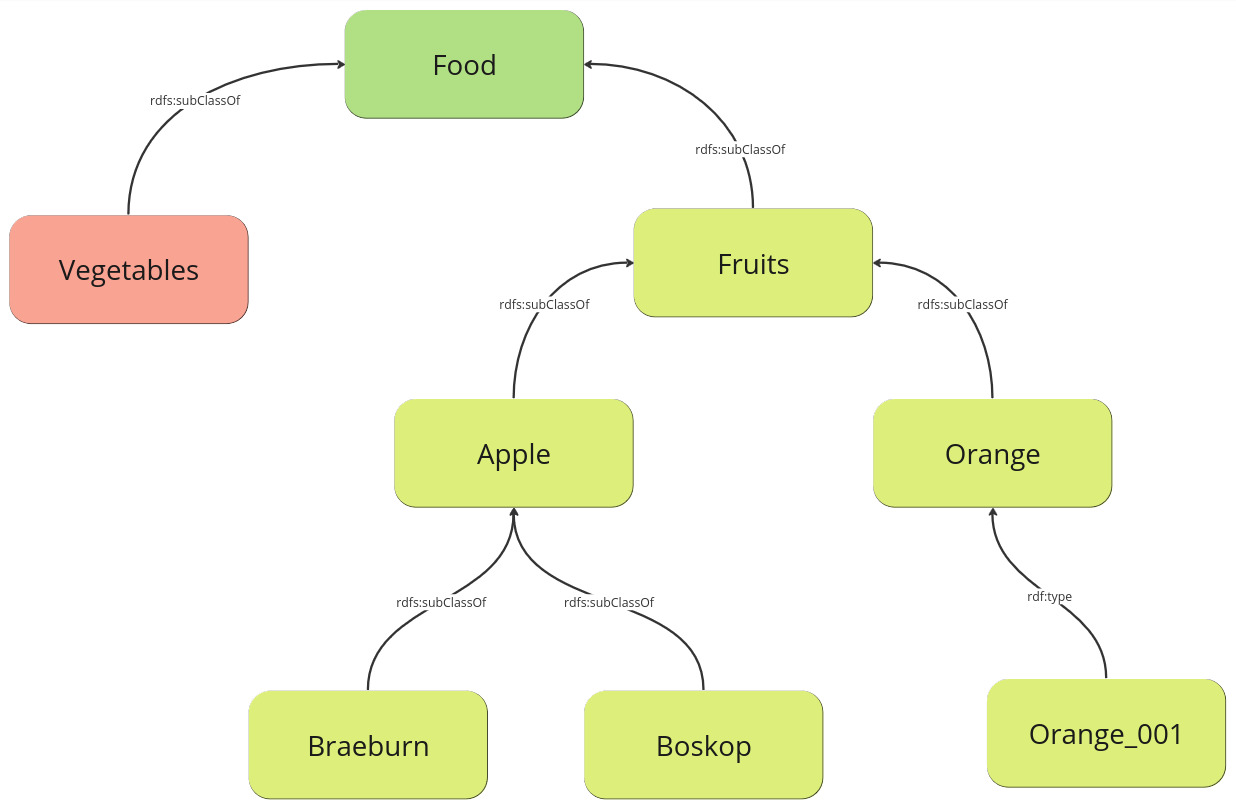
\includegraphics[scale=0.8]{Graphics/ontology.jpg}
        \end{figure}
	Key components of ontologies include:

	\begin{itemize}
		\item Concepts/Classes: These represent abstract or concrete entities within a domain. For example, in a medical ontology, "Patient" and "Disease" might be classes.
		\item Properties/Roles: These define the relationships between concepts. For instance, in a social network ontology, "FriendOf" could be a property connecting individuals.
		\item Instances/Individuals: These are specific members or examples of a class. In a geographical ontology, "New York City" and "Paris" could be instances of the class "City."
		\item Axioms: These are statements that describe the properties and relationships of the entities within the ontology. Axioms help define the logic and rules governing the domain.
		\item Hierarchy: Ontologies often organize concepts into a hierarchy, with more general concepts at the top and more specific ones below. This hierarchical structure aids in categorization and understanding.
		\item Inference Rules: These rules define how new information can be derived from existing information in the ontology. Inferences help systems reason and make deductions based on the knowledge encoded in the ontology.
	\end{itemize}
	We utilize ontologies in knowledge representation and reasoning systems to empower the robot with the ability to comprehend and handle information in a structured fashion for our specific objectives.

	\subsection*{SWRL}
	SWRL, which stands for Semantic Web Rule Language, is a rule language that allows users to define rules about the relationships between classes and individuals in ontologies represented in the Web Ontology Language (OWL). SWRL is part of the W3C's Semantic Web technology stack and is designed to be used in conjunction with OWL to express complex relationships and infer new information based on existing knowledge.

	SWRL Rules have a specific syntax and consist of two main components:
	\begin{itemize}
		\item Antecedent (Body): This part of the rule specifies the conditions or constraints that must be satisfied for the rule to be applicable. It describes the current state of the ontology that triggers the rule.
		\item Consequent (Head): This part defines the actions or inferences that should be taken if the conditions specified in the antecedent are satisfied. It describes the changes or additional information that should be inferred when the rule is triggered.
	\end{itemize}
	SWRL supports various built-in predicates and functions, and users can create their own custom rules to suit their specific ontology. Some common elements in SWRL rules include:
	\begin{itemize}
		\item Individuals: Refers to specific instances of classes in the ontology.
		\item Class and Property Relationships: Describes relationships between classes and properties in the ontology.
		\item Built-in Predicates and Functions: Includes operations such as arithmetic, string manipulation, and comparison functions that can be used in the rule conditions.
	\end{itemize}
	Here's a simple example of a SWRL rule:
	\newline
	$Person(?x) ^ hasChild(?x, ?y) -> Grandparent(?x, ?z) ^ hasChild(?y, ?z)$
	\newline
	In this example:

	If an individual (?x) is a Person and has a child (?y),
	
	Then, infer that the individual (?x) is a Grandparent of another individual (?z), and the child (?y) is the parent of (?z).
	
	SWRL rules are useful for expressing complex relationships and constraints within ontologies, enabling automated reasoning systems to make inferences and derive new knowledge from existing data.
	\section*{Libraries}
	\subsection*{OWLReady}
	One important library used for our Implementation is OWLReady. "OWLReady" is a Python library designed for ontology-oriented programming. It facilitates the development, manipulation, and querying of ontologies using the Web Ontology Language (OWL), a standard for representing knowledge in a machine-readable format. OWLReady simplifies ontology-related tasks by providing a convenient and object-oriented interface for working with OWL ontologies in Python.

	Key features of the OWLReady library include:

	\begin{itemize}
		\item Object-Oriented Programming (OOP): OWLReady adopts an object-oriented approach, allowing users to interact with ontology entities as Python objects. This makes it more intuitive for developers familiar with Python's OOP principles.
		\item Ontology Loading and Parsing: The library supports the loading and parsing of OWL ontologies, making it easy to access and manipulate ontology data within Python scripts or applications.
		\item Class and Individual Manipulation: OWLReady provides functionality for creating, modifying, and querying classes and individuals within an ontology. This allows for dynamic and programmatic management of ontology content.
		\item Reasoning Support: Depending on the version and features, OWLReady may offer support for reasoning tasks. Reasoning involves deducing implicit information based on the logical relationships defined in the ontology.
		\item Integration with RDFLib: OWLReady may integrate with RDFLib, another Python library commonly used for working with Resource Description Framework (RDF) data. This integration enhances the capabilities of handling semantic data.
	\end{itemize}
	\newpage
	\subsection*{WikiHow}
	
	\begin{wrapfigure}{r}{0.5\textwidth}
        \centering
        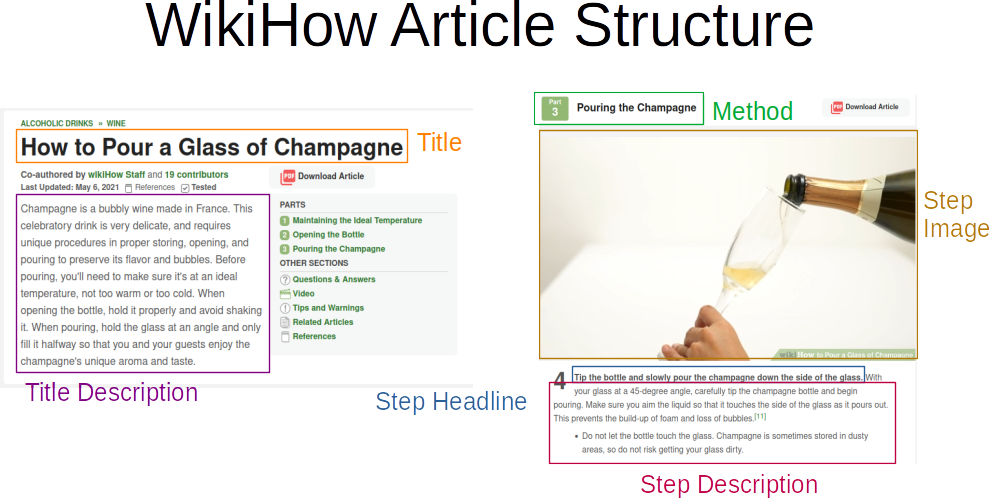
\includegraphics[width=0.48\textwidth]{Graphics/WikiHow Article Structure.png}
    \end{wrapfigure}
	WikiHow is an extraction tool, that can collect informations from the WikiHow Corpus. The goal of this tool is to analyse a WikiHow corpus using basic NLP techniques to gather information about Everyday tasks like "Pouring", "Cutting" or "Discarding". These information should support cognitive robots in understanding and parameterizing these tasks to better handle unknown tasks, working in underspecified environments and handling common task-object combinations.
	Jedes Verb hat eine eigene Klasse, worin das Verb und die zusätzlich gewünschten Hyponyme/Synonyme definiert sind. Diese Verben dienen das als Schlüsselwort, wonach in den WikiHow Artikeln letzendlich gesucht wird. Außerdem kann man verschiedene Parameter einstellen, wie zum Beispiel das Ausschließen verschiedener Kategorien, welche für die Suche nicht von Relevanz sind.